\documentclass[11pt]{article}

\usepackage[margin=1in]{geometry}
\usepackage[T1]{fontenc}
\usepackage{lmodern}
\usepackage{microtype}
\usepackage{graphicx}
\usepackage{booktabs}
\usepackage{longtable}
\usepackage{amsmath}
\usepackage{xcolor}
\usepackage{caption}
\usepackage{subcaption}
\usepackage{enumitem}
\usepackage[section]{placeins}
\usepackage[colorlinks=true,linkcolor=blue!50!black,urlcolor=blue!50!black,citecolor=blue!50!black]{hyperref}

\graphicspath{{figures/}}
\captionsetup{font=small,labelfont=bf}
\setlist{itemsep=2pt,topsep=4pt}

% Highlighted boxes for the parts only the author can write. Search for
% "\yours" to find them all; delete the macro calls once they are filled in.
\newcommand{\yours}[1]{\par\smallskip\noindent\colorbox{yellow!25}{\parbox{\dimexpr\linewidth-2\fboxsep}{\small\textbf{Fill in:} #1}}\par\smallskip}

\newcommand{\rl}[1]{\texttt{#1}}
\newcommand{\website}{\url{https://yoshijoshi21.github.io/Game-of-Life-3D/}}
\newcommand{\repo}{\url{https://github.com/YoshiJoshi21/Game-of-Life-3D}}

\title{Emergent Complexity in Outer-Totalistic Cellular Automata\\[4pt]\large A 2D/3D simulator, a survey of random rules, and a look at 3D life}
\author{\colorbox{yellow!25}{Fill in: your name}}
\date{September 2026}

\begin{document}
\maketitle

\begin{abstract}
I built an interactive cellular-automaton lab: a C++ engine for binary outer-totalistic rules in 2D (8 neighbours) and 3D (26 neighbours), a classifier that sorts rules into stable, oscillating, chaotic and complex, and a website that runs both in the browser through WebAssembly. With it I ran 144 random Life soups and 144 HighLife soups to see what is left behind, surveyed 100 (and then 1000) random 2D rules, and took the 3D extension. The main findings: Life's settled ``ash'' is about 2.85\% live cells from almost any starting density. HighLife's replicator copies itself in a Sierpinski pattern: the population at generation $12k$ is exactly $12\cdot 2^{\mathrm{popcount}(k)}$. Among random rules, whether the rule contains a low birth count (B0, B1 or B2) predicts chaos far better than Langton-style $\lambda$ does. And in 3D, uniformly random rules are \emph{all} chaotic, because 97\% of them contain a birth count of 4 or less; sparser sampling brings stable rules back, split almost perfectly by the smallest birth count.
\end{abstract}

\begin{center}
\footnotesize
\begin{tabular}{@{}ll@{}}
Website & \website \\
Code    & \repo \\
Reproduce the numbers & \texttt{g++ -O3 -std=c++17 experiments/experiments.cpp -o experiments/run} \\
                      & \texttt{./experiments/run all \&\& python3 experiments/figures.py} \\
\end{tabular}
\end{center}

\tableofcontents
\bigskip

%=====================================================================
\section{What I built and how it works}
%=====================================================================

\subsection{The simulation engine (C++)}

All simulation code sits behind one interface, \texttt{LifeGame} (\texttt{engine/lifeGame.hpp}), with two implementations:

\begin{itemize}
  \item \texttt{LifeGrid} (\texttt{engine/life.hpp}): a $W\times H$ grid of cells, each on or off. The edges wrap around (a torus), so there are no borders.
  \item \texttt{LifeGrid3D} (\texttt{engine/life3D.hpp}): the same for a $W\times H\times D$ grid, with the 26-cell Moore neighbourhood.
\end{itemize}

A rule is a list of birth counts $B$ and survival counts $S$. When the rule is set, each class builds two lookup tables, \texttt{canBirth[n]} and \texttt{canSurvive[n]} for $n=0\ldots8$ (or $0\ldots26$). Then \texttt{step()} is one loop: count the live neighbours of every cell, look up the next state, write it into a second buffer, and swap the two buffers. Both classes expose \texttt{flatten()}, which returns one byte per cell with index $(z\cdot H + y)\cdot W + x$. The classifier and the website both read the grid through this.

\subsection{The classifier (\texttt{analysis/analysis.hpp})}

\texttt{Analysis::classify} runs a rule from several random starting grids (``soups''), one per starting density, and labels each run:

\begin{enumerate}
  \item Each generation, the whole grid is hashed (64-bit FNV-1a over \texttt{flatten()}), and the generation at which each hash was first seen is stored. When a hash repeats, the run is periodic from then on. A period of 1 means \textbf{stable}; anything longer means \textbf{oscillating}. The code records the period and the generation of the first repeat.
  \item If nothing repeats within \texttt{maxGen} generations, the run is \textbf{chaotic} or \textbf{complex}. To tell them apart, it averages over the last 50 generations the Shannon entropy of the live fraction in every $5\times5$ (or $5\times5\times5$) window, $H(p) = -p\log_2 p - (1-p)\log_2(1-p)$. The windows are summed one axis at a time so the cost stays linear. Mean entropy above 0.35 counts as chaotic (well-mixed noise everywhere); below that counts as complex (activity with structure and empty space).
  \item The rule's label is a majority vote over its runs. Ties go to the more interesting category.
\end{enumerate}

\texttt{analysis/main.cpp} samples random rules and prints this for each one. A rule is a random 64-bit number from \texttt{mt19937\_64}, masked to $2(N+1)$ bits: the low $N+1$ bits are the birth counts and the next $N+1$ are the survival counts. Duplicates are skipped.

\subsection{The website}

The website (Figure~\ref{fig:site}) runs the same C++ in the browser. \texttt{wasm/bindings.cpp} wraps the engine and the classifier, and Emscripten compiles them to WebAssembly (\texttt{build.sh}). Nothing in \texttt{engine/} or \texttt{analysis/} had to change for the web. The site has three parts.

\paragraph{Viewer.} Play, pause, single step, reset to generation~0, clear, and a speed slider from 1 generation per second up to ``as fast as possible''. You can draw by clicking or dragging (starting on a live cell erases), or stamp known patterns (glider, LWSS, Gosper gun, HighLife replicator\ldots). Cells are coloured by age: a cell that was just born or just drawn is white, and it cools through sky blue to deep blue as it survives. Dead cells leave a short fading trail. This makes motion easy to see: gliders show up as white fronts, and still lifes turn dark blue. A sparkline under the grid plots the population over time.

\paragraph{Rule editor.} Birth and survival are two rows of toggle chips. In 2D each chip shows a small $3\times3$ neighbourhood with $n$ neighbours lit, so the meaning of each count is visible. The rule string can also be typed (\rl{B36/S23}, \rl{B5/S4,5}, \rl{B13-14,17-19/S13-26}) or picked from presets. A sentence under the chips states the rule in plain English and warns about B0 strobing.

\paragraph{3D editor.} The 3D grid is drawn with three.js as instanced cubes (one draw call for every live cell), with the same age colours. You orbit, zoom and pan the camera with the mouse. To edit, you either click a cube face, which stacks a new cell on that face, or click the translucent ``layer'' plane to place a cell on that layer. \texttt{[} and \texttt{]} move the layer, and a cut-away option hides everything above it so the inside can be edited. Picking uses a voxel ray-march (Amanatides--Woo) through the grid rather than testing the ray against every cube, so it stays fast with tens of thousands of cells.

\paragraph{Rule survey.} This runs the \texttt{main.cpp} survey in the browser, spread across one web worker per CPU core. It shows category counts, a $\lambda$ vs.\ final-density scatter, a histogram of when runs first repeated, and a card per rule with thumbnails of each run's final grid. Clicking a card replays that exact run (same grid size, density and seed) in the viewer. Results can be exported as CSV.

The survey had one design problem. \texttt{Analysis} draws every run's random seed from one generator, in order, so rule \#57's seeds depend on having run rules \#1--56 first. That rules out running rules in parallel. The fix was a small wrapper game (\texttt{SeededGame}) that passes everything through to the real grid, except that \texttt{randomize()} swaps in the seed that rule would have received in the sequential run. The survey can then run on every core and still reproduce the CLI exactly. With seed 2026 and the CLI's settings, the website lists the same 100 rules with the same labels and entropies.

\begin{figure}[!htbp]
  \centering
  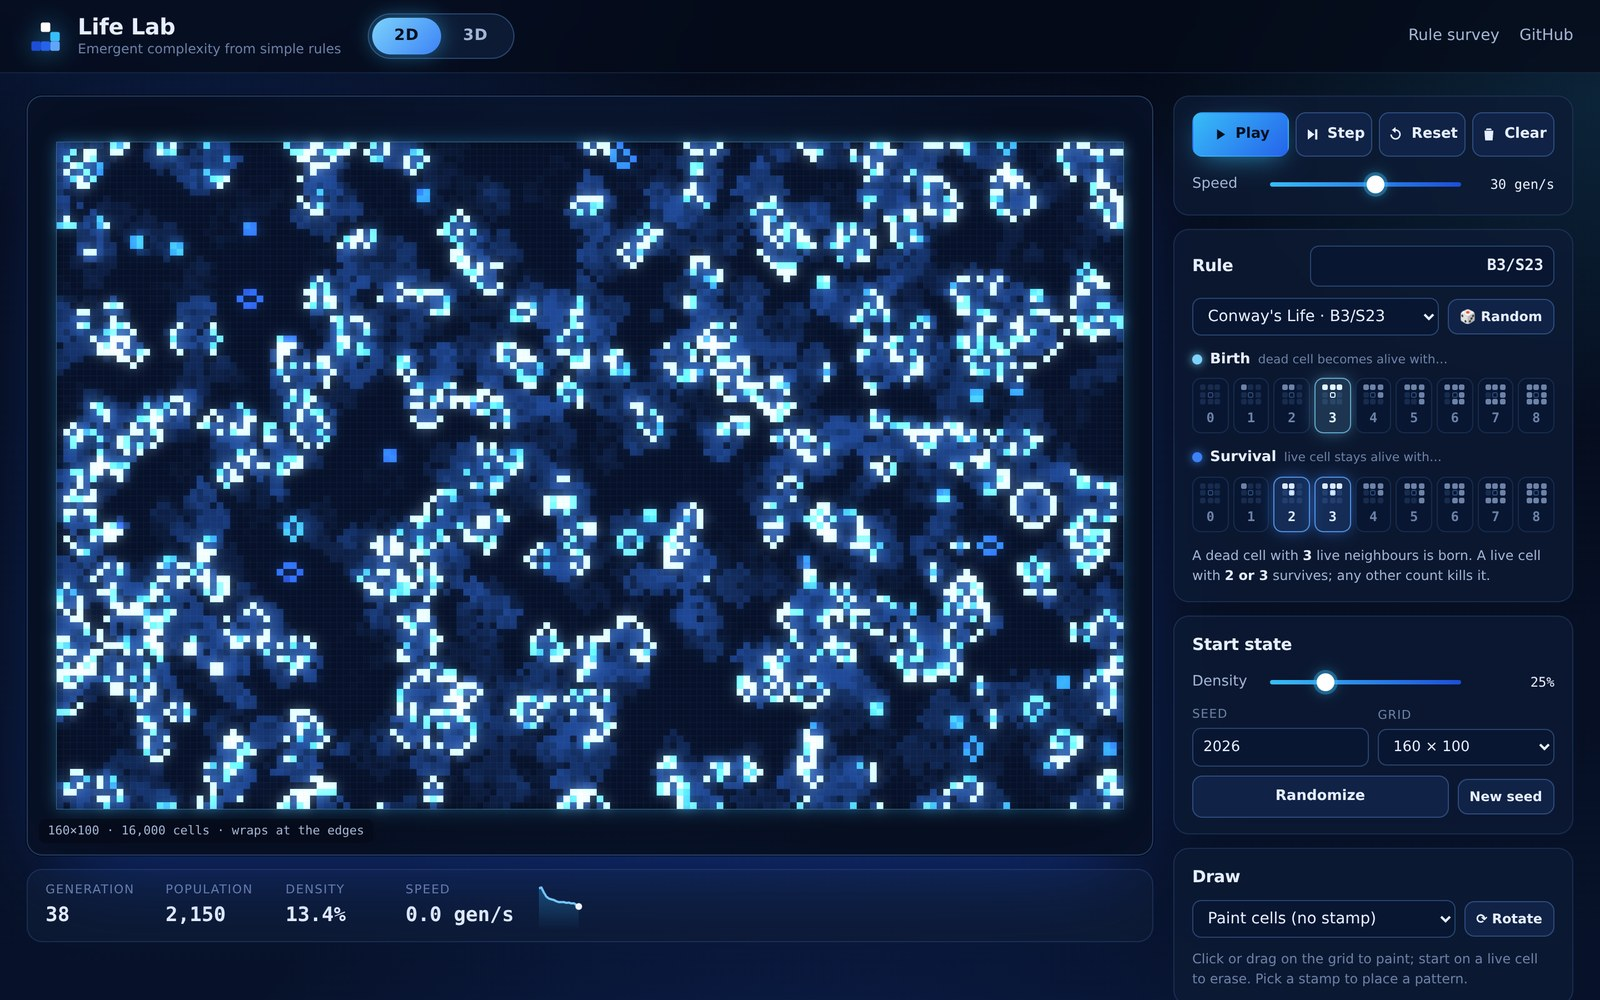
\includegraphics[width=\linewidth]{site_2d.jpg}\\[4pt]
  \begin{subfigure}[t]{0.36\linewidth}\centering
    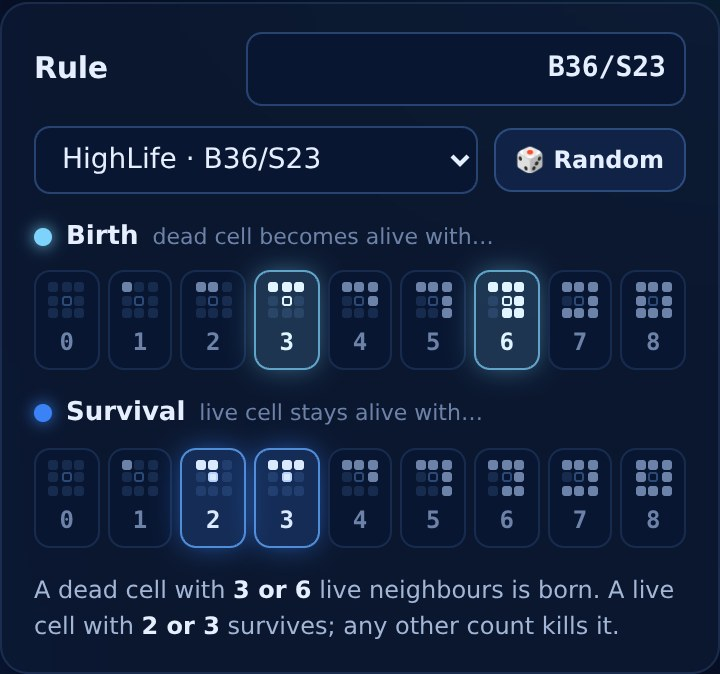
\includegraphics[width=\linewidth]{site_rule_editor.jpg}
    \caption{Rule editor with HighLife selected.}
  \end{subfigure}\hfill
  \begin{subfigure}[t]{0.61\linewidth}\centering
    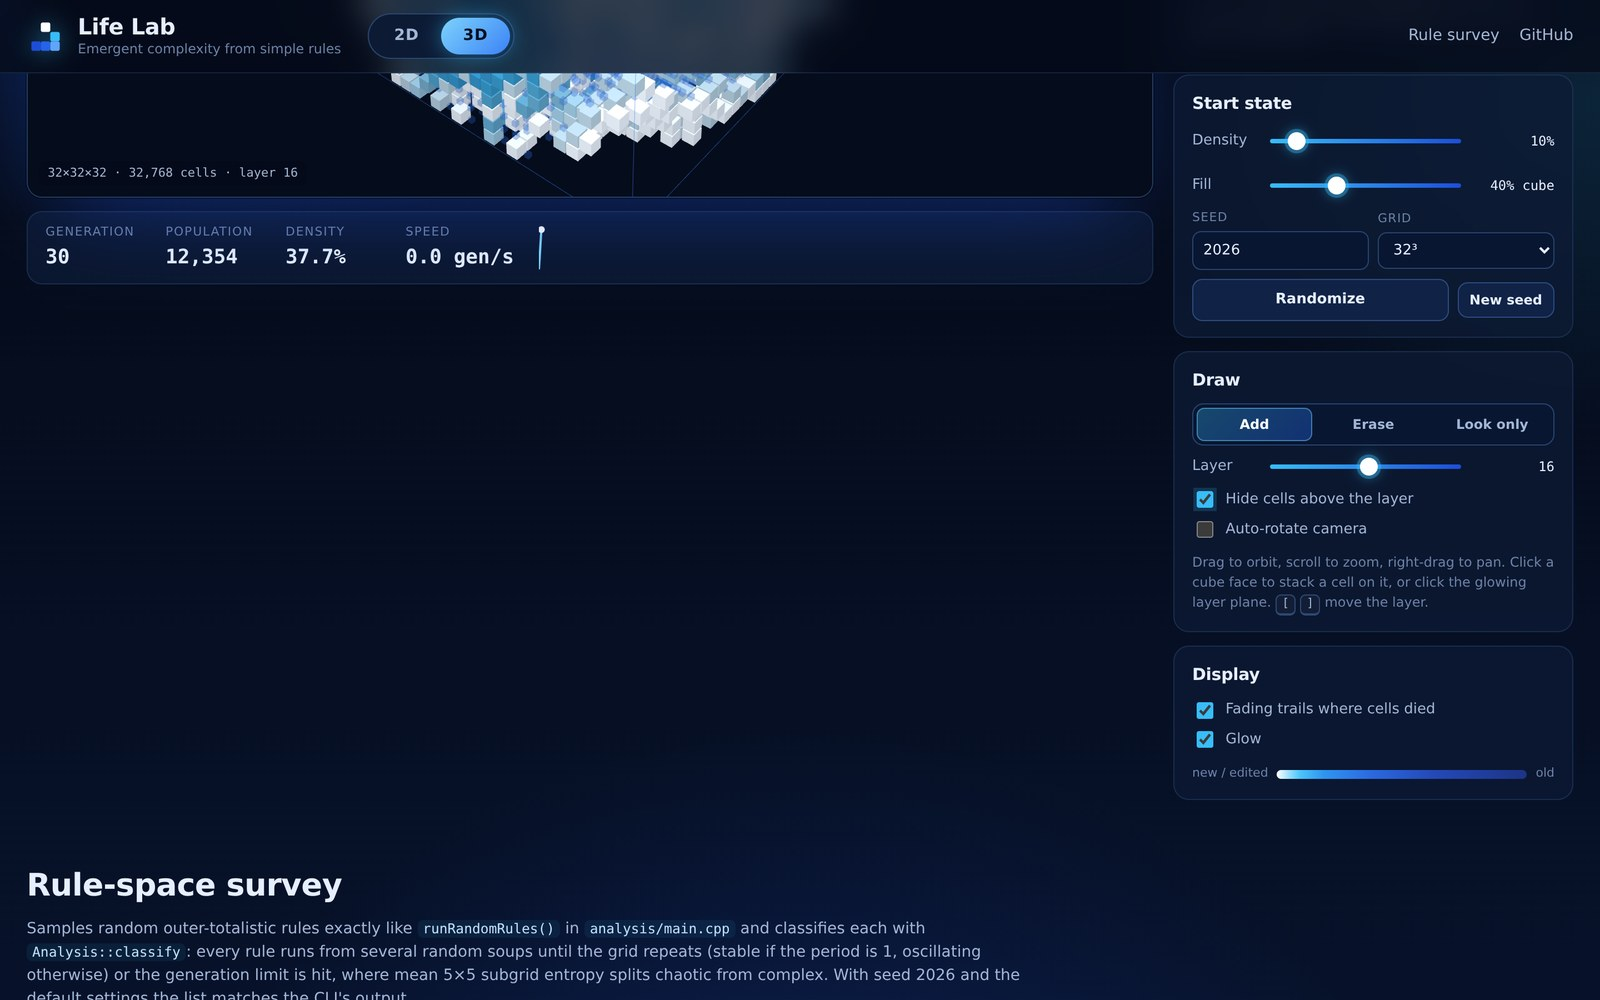
\includegraphics[width=\linewidth]{site_3d_edit.jpg}
    \caption{3D editor: layer plane, cut-away, hover cursor.}
  \end{subfigure}
  \caption{The website. Top: Life from a random soup. New cells are white and older cells are darker blue, with faint trails where cells died.}
  \label{fig:site}
\end{figure}

\subsection{Design decisions}

\begin{itemize}
  \item \textbf{Torus boundaries.} There are no edge effects and every cell has a full neighbourhood. The cost is that gliders loop forever and eventually crash into the debris they left behind (Section~\ref{sec:life}).
  \item \textbf{Cycle detection by hashing the whole grid.} This catches any period with no extra bookkeeping. A 64-bit hash could in principle collide and fake a cycle, but with at most a few thousand states per run that chance is negligible.
  \item \textbf{WebAssembly instead of a JavaScript rewrite.} The website and the experiments run the same code, so what you see in the browser is what the report measures.
  \item \textbf{Instanced cubes for 3D.} One draw call handles every live cell. Only the positions and colours of live cells are uploaded each frame.
\end{itemize}

%=====================================================================
\section{Questions}
%=====================================================================

\begin{enumerate}
  \item What does Conway's Life turn into from random soups, and how does that depend on the starting density?
  \item Which objects appear, and how often? How does HighLife (\rl{B36/S23}) differ?
  \item Among random outer-totalistic rules, how common are stable, oscillating, chaotic and complex behaviour? What about a rule predicts its category?
  \item What is going on in the rules the classifier calls ``complex''?
  \item In 3D: what do random rules do, how does that compare with 2D, and how big a grid is practical?
\end{enumerate}

%=====================================================================
\section{Task 1: Conway's Life from random soups}\label{sec:life}
%=====================================================================

\paragraph{Setup.} $128\times128$ torus, rule \rl{B3/S23}. Twelve starting densities (0.05 to 0.4 in steps of 0.05, then 0.5, 0.6, 0.7 and 0.8), with 12 seeds each, for 144 soups. Each soup runs until its state repeats, or for at most 6000 generations. At the end I split the grid into 8-connected clusters and identify each one up to rotation and reflection. To name them, I ran known patterns (block, beehive, glider, toad, \ldots) through the engine, recording every phase.

\begin{figure}[!htbp]
  \centering
  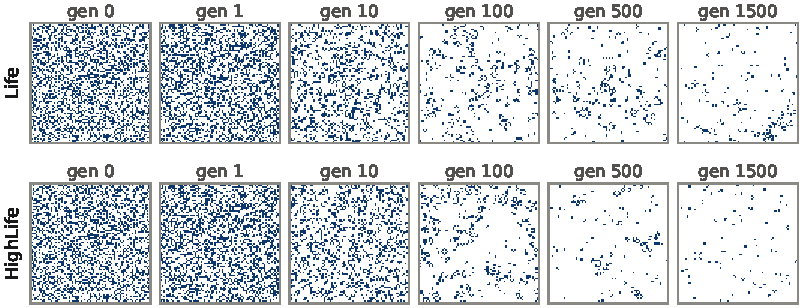
\includegraphics[width=\linewidth]{soup_snapshots.pdf}
  \caption{The same $d=0.35$ soup (seed 7) under Life (top) and HighLife (bottom), at generations 0, 1, 10, 100, 500 and 1500.}
  \label{fig:snapshots}
\end{figure}

\paragraph{Three phases.} Every soup went through the same three stages (Figures~\ref{fig:snapshots} and~\ref{fig:traces}):
\begin{enumerate}
  \item \textbf{Die-off} (first 10 generations). Crowded and isolated cells die at once. For starting densities 0.15--0.6 the density lands between 0.10 and 0.24 by generation 10, much closer together than where they started. Very sparse (0.05) and very dense ($\ge0.7$) soups lose almost everything here.
  \item \textbf{Long transient} (hundreds to thousands of generations). The grid becomes an archipelago of active regions. Blobs grow, collide and burn out; gliders leave and later hit something; and regions that seemed dead get restarted by debris. The population drifts down slowly with bursts.
  \item \textbf{Ash.} Only still lifes and period-2 oscillators remain. 136 of the 144 soups ended with period exactly 2 (blinkers, toads and beacons flipping among still lifes).
\end{enumerate}

\begin{figure}[!htbp]
  \centering
  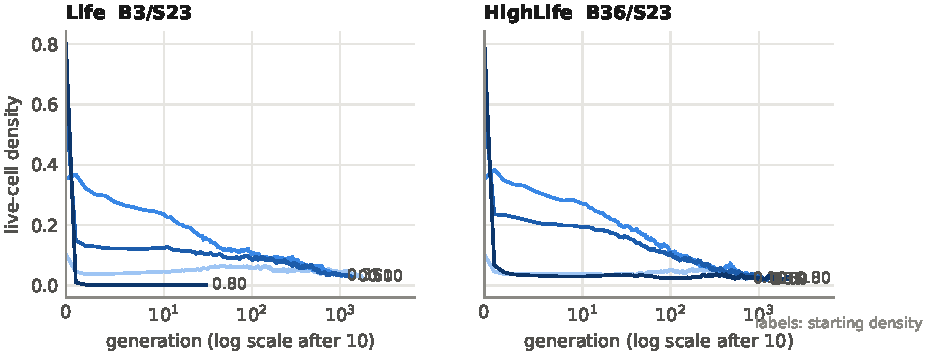
\includegraphics[width=\linewidth]{soup_traces.pdf}
  \caption{Live-cell density over time for one soup at four starting densities (seed 0). The generation axis is logarithmic after 10.}
  \label{fig:traces}
\end{figure}

\paragraph{How long and how much.} For starting densities 0.1--0.7, the median time to the first repeated state is 1200--2600 generations, with a wide spread (Figure~\ref{fig:settling}, left). The settled ash is remarkably consistent: \textbf{$2.85\% \pm 0.32\%$ live cells} (mean $\pm$ s.d.\ over 120 soups) for any starting density from 0.1 to 0.7. The extremes behave differently. At $d=0.05$ most cells are isolated and die, and soups settle by about generation 67 (median) with 0.8\% ash. At $d=0.8$ almost every cell is overcrowded and dies in the first step, so soups settle by generation 12 with 0.2\% ash.

\begin{figure}[!htbp]
  \centering
  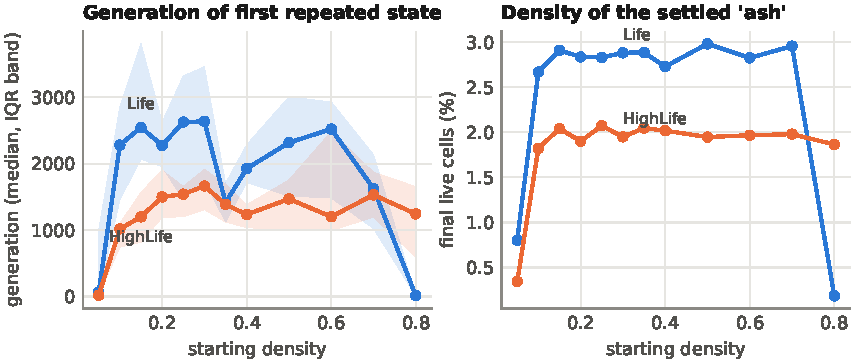
\includegraphics[width=\linewidth]{soup_settling.pdf}
  \caption{Left: generation of the first repeated state (median of 12 soups; band = interquartile range). Right: mean density of the final ash.}
  \label{fig:settling}
\end{figure}

\paragraph{What is left.} Figure~\ref{fig:census} counts the 7{,}702 objects left by the 48 soups with $d\in[0.2,0.5]$. Blinkers (33.8\%), blocks (32.2\%) and beehives (19.0\%) make up 85\% of all objects. They are followed by loaves, boats, ponds, tubs, ships, toads, long boats, beacons and barges. Only 0.4\% of clusters were unnamed; these were larger still lifes, or two still lifes touching diagonally, which counts as one cluster.

\paragraph{Moving objects.} Gliders are everywhere during the transient, but on a torus a glider can't escape. Three soups ended with a period of \textbf{512} $= 4\times128$: the time it takes a glider (speed $c/4$ diagonally) to go round the $128\times128$ torus once. In each case the glider had found a clear lane through the ash. Four soups (all $d\ge0.5$) were still active at generation 6000.

\yours{Add a few structures you noticed yourself on the website, with screenshots: for example a glider leaving a blob, the ``traffic light'' (four blinkers), or a pulsar forming from a soup. Say what you found surprising.}

%=====================================================================
\section{Task 2: an editable rule and HighLife}
%=====================================================================

The rule editor is described in Section~1.3. Clicking the ``6'' chip in the birth row turns Life into HighLife (\rl{B36/S23}). The one difference: a dead cell with six live neighbours is also born.

\paragraph{HighLife soups.} I repeated the soup experiment with \rl{B36/S23} (Figures~\ref{fig:snapshots} and~\ref{fig:census}). HighLife looks almost the same as Life for most of the run, but the statistics differ:
\begin{itemize}
  \item The ash is thinner: \textbf{$1.97\%\pm0.22\%$} live cells, against 2.85\% for Life.
  \item The mix of objects is different. Blocks are 42\% of objects (32\% in Life), and blinkers only 15\% (34\% in Life). Loaves and boats are more common.
  \item \textbf{Dense soups do not die.} At $d=0.8$, Life dies in about 12 generations, but HighLife soups ran for a median of 1244 generations and left 1.9\% ash. B6 lets new cells appear inside a crowded region, so the initial die-off leaves seeds behind instead of nothing.
  \item All 144 soups settled. One ended with a \textbf{period-14} cycle, the only period in HighLife other than 1 or 2.
\end{itemize}

\begin{figure}[!htbp]
  \centering
  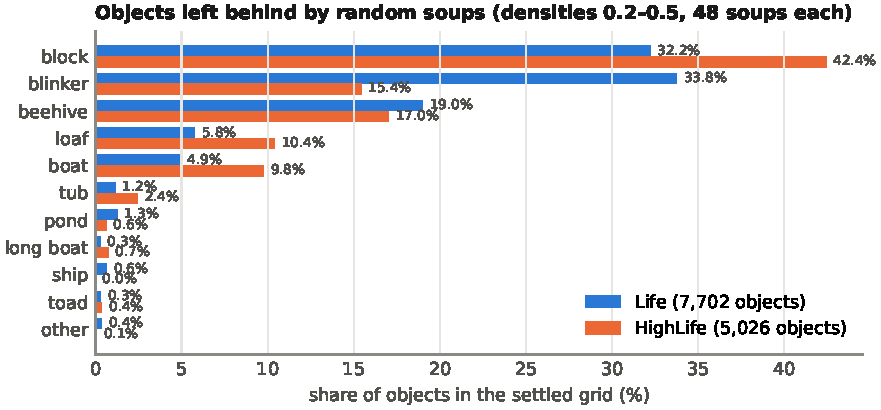
\includegraphics[width=\linewidth]{census.pdf}
  \caption{Census of the settled grids of 48 soups per rule. Toads and beacons split into two pieces in one phase; the census recognises this and counts them as whole objects.}
  \label{fig:census}
\end{figure}

\paragraph{The replicator.} HighLife is famous for its \emph{replicator}, a 12-cell pattern that makes copies of itself. I placed one on a $320\times320$ torus, large enough that the copies don't wrap round within 300 generations, and tracked it (Figure~\ref{fig:replicator}). Every 12 generations the pattern consists of whole copies of the replicator lined up on a diagonal. Where two copies would land on the same spot, they destroy each other. The copy count follows the Sierpinski triangle, like the elementary cellular automaton rule 90 (XOR of the two neighbours). At generation $12k$ the population is exactly
\[
  \text{population}(12k) = 12\cdot 2^{\,\mathrm{popcount}(k)},
\]
where $\mathrm{popcount}(k)$ is the number of 1 bits in $k$. I checked this for every $k=0,\ldots,24$ and all 25 values match. For example, $k=15=1111_2$ gives 16 copies (192 cells), and $k=16=10000_2$ gives just 2 (24 cells).

\begin{figure}[!htbp]
  \centering
  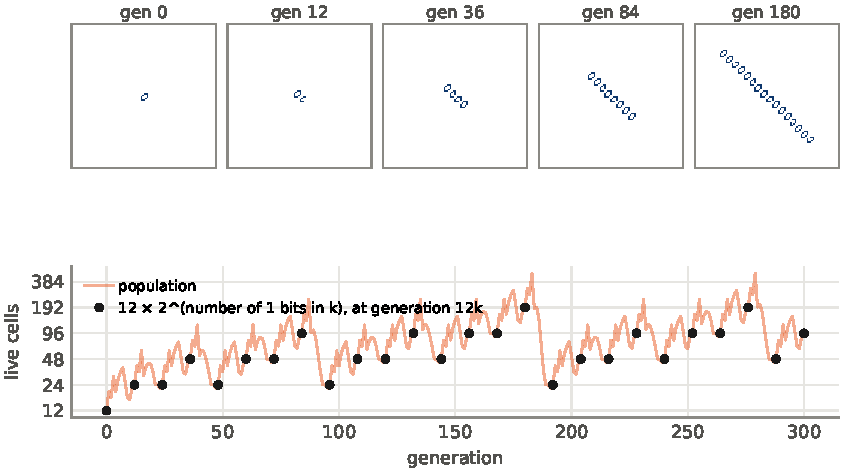
\includegraphics[width=\linewidth]{replicator.pdf}
  \caption{The HighLife replicator. Top: generations 0, 12, 36, 84 and 180 (1, 2, 4, 8 and 16 copies), each shown in the same $100\times100$ window. Bottom: population (orange) and the prediction $12\cdot2^{\mathrm{popcount}(k)}$ at every 12th generation (black).}
  \label{fig:replicator}
\end{figure}

\paragraph{Catalogue of HighLife patterns found.}
\begin{center}\small
\begin{tabular}{@{}lll@{}}
\toprule
Kind & Patterns & How found \\
\midrule
Still lifes & block, beehive, loaf, boat, tub, pond, barge, long boat & soup census \\
Oscillators & blinker, toad, beacon (period 2); one period-14 & soup census \\
Spaceships & glider (same as Life's; checked with the engine) & soups, stamp \\
Replicator  & 12-cell replicator, Sierpinski growth & stamp (website) \\
\bottomrule
\end{tabular}
\end{center}

\yours{Add any HighLife patterns you found by hand on the website (e.g.\ by stamping two replicators near each other, or a replicator next to a block).}

%=====================================================================
\section{Task 3: 100 random rules}
%=====================================================================

\paragraph{Setup.} Exactly as \texttt{main.cpp}: 100 distinct rules drawn uniformly from all $2^{18}$ (seed 2026), each run on a $64\times64$ torus for at most 500 generations from starting densities 0.2, 0.35 and 0.5, then classified by majority vote. To check that 100 rules is enough, I also classified a second, independent sample of 1000 rules (seed 7) with the same settings. Appendix~\ref{app:table} lists all 100 rules and their three runs.

\begin{figure}[!htbp]
  \centering
  \begin{minipage}[b]{0.46\linewidth}
    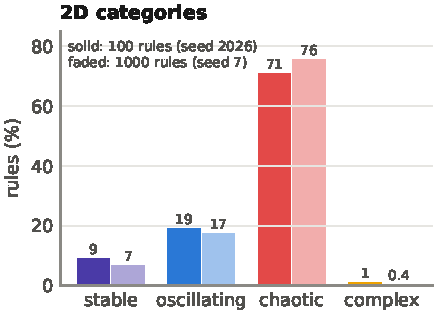
\includegraphics[width=\linewidth]{survey_categories.pdf}
  \end{minipage}\hfill
  \begin{minipage}[b]{0.52\linewidth}
    \small
    \begin{tabular}{@{}lrr@{}}
      \toprule
      & 100 rules & 1000 rules \\
      \midrule
      stable      &  9 & 66 (6.6\%) \\
      oscillating & 19 & 173 (17.3\%) \\
      chaotic     & 71 & 757 (75.7\%) \\
      complex     &  1 & 4 (0.4\%) \\
      \midrule
      runs disagree & 9 & 60 \\
      \bottomrule
    \end{tabular}
    \vspace{12pt}
  \end{minipage}
  \caption{Categories of random 2D rules. ``Runs disagree'' counts rules whose three runs did not all get the same label.}
  \label{fig:categories}
\end{figure}

\paragraph{The categories.} The 100-rule sample gave 9 stable, 19 oscillating, 71 chaotic and 1 complex rule, and the 1000-rule sample confirms those shares (Figure~\ref{fig:categories}). Figure~\ref{fig:thumbs} shows typical end states:
\begin{itemize}
  \item \textbf{Stable} rules either freeze almost at once into a mesh of still cells (\#18, \#35) or die out apart from a few tiny still lifes (\#9). Four of the 1000 rules killed every cell in all three runs.
  \item \textbf{Oscillating} rules mostly have period 2. Across the 1000-rule sample the most common periods were 2 (227 runs), 4 (79), 12 (69) and 6 (57), with a few long ones (60, 84). Many period-2 rules are \emph{strobing}: they contain B0 (an empty neighbourhood gives birth) but not S8 (a full neighbourhood doesn't survive), so the whole grid inverts every step.
  \item \textbf{Chaotic} rules fill the grid with noise and never repeat. Their mean entropy ranged from 0.49 to 0.99.
  \item \textbf{Complex} was very rare: 1 in 100 and 4 in 1000. Section~\ref{sec:strobe} looks at why.
\end{itemize}

\begin{figure}[!htbp]
  \centering
  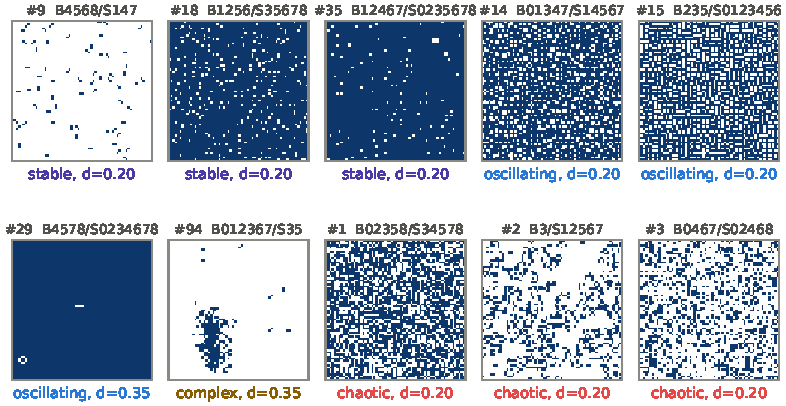
\includegraphics[width=\linewidth]{survey_thumbnails.pdf}
  \caption{Final grids ($64\times64$) of some of the 100 sampled rules, shown for the run that agreed with the rule's vote.}
  \label{fig:thumbs}
\end{figure}

\paragraph{What predicts the category?} Langton's $\lambda$ for general CA is the fraction of rule-table entries that lead to a live cell. For outer-totalistic rules the analogue is $\lambda=(|B|+|S|)/2(N+1)$. In this sample it does not separate the categories at all: the median $\lambda$ is 0.50 for stable, oscillating and chaotic rules alike (Figure~\ref{fig:lambda}). The \emph{smallest birth count} is a much better predictor (Figure~\ref{fig:birth}). If a rule lets a dead cell be born with 0, 1 or 2 neighbours, it is chaotic 77--85\% of the time: small birth counts fire everywhere in a sparse grid, so activity never runs out. Of the rules whose lowest birth count is 3 or more (like Life), only 39\% are chaotic, and 30\% are stable and 29\% oscillating. Since each count is in $B$ with probability $\tfrac12$, only $1/8$ of uniformly random rules avoid B0, B1 and B2. That is the main reason chaos dominates the sample.

\begin{figure}[!htbp]
  \centering
  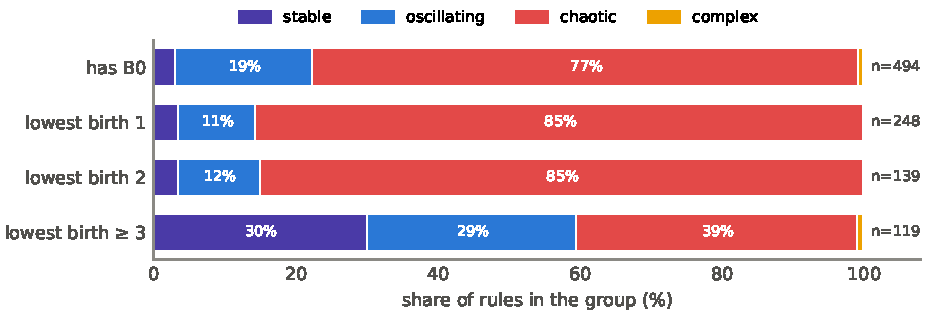
\includegraphics[width=\linewidth]{survey_birth.pdf}
  \caption{1000 random 2D rules, grouped by their smallest birth count.}
  \label{fig:birth}
\end{figure}

\begin{figure}[!htbp]
  \centering
  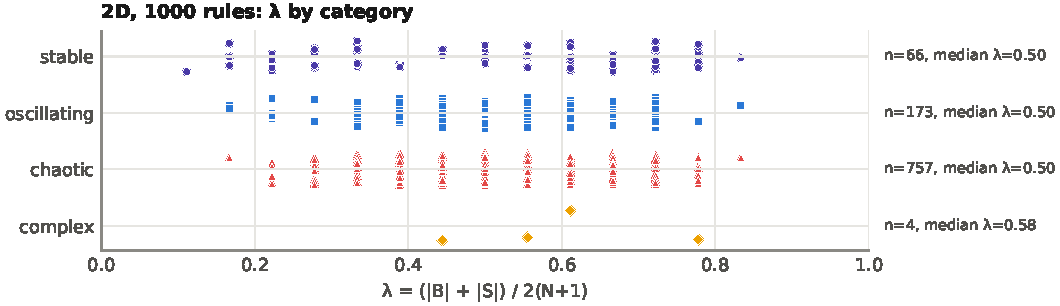
\includegraphics[width=\linewidth]{survey_lambda.pdf}
  \caption{$\lambda$ for the 1000-rule sample, one mark per rule. The categories overlap almost completely.}
  \label{fig:lambda}
\end{figure}

\paragraph{One run is not enough.} 9 of the 100 rules (60 of 1000) got different labels from different starting densities. The most common splits were stable/oscillating (28 rules), chaotic/oscillating (15) and complex/oscillating (14). The lowest density often settles while higher densities keep going. The same rule really can behave differently depending on where it starts.

\subsection{A closer look: the ``complex'' rule \rl{B012367/S35}}\label{sec:strobe}

The only complex rule in the 100-rule sample was \#94, \rl{B012367/S35}. Its runs were: oscillating with period 2 (first repeat at generation 272) from $d=0.2$, and complex with $H=0.133$ and $H=0.224$ from $d=0.35$ and $0.5$. Watching it on the website shows why the entropy is low (Figure~\ref{fig:strobe}): the grid \emph{strobes}. On even generations the density falls towards 10--15\%; on odd generations it rises towards 85--90\%. Large regions go almost uniform, which gives low local entropy.

\begin{figure}[!htbp]
  \centering
  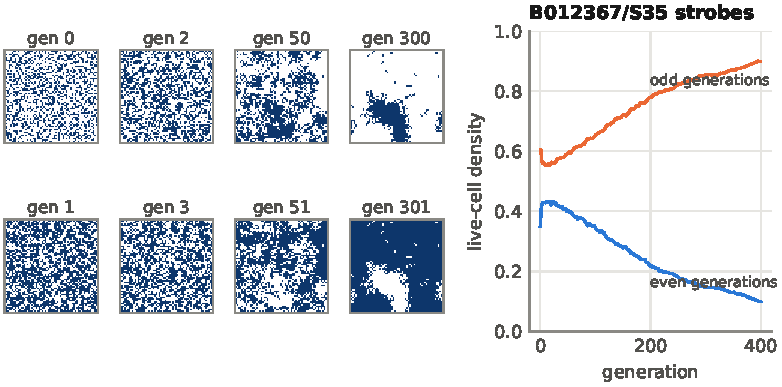
\includegraphics[width=\linewidth]{strobe.pdf}
  \caption{\rl{B012367/S35} from a $d=0.35$ soup on $128\times128$ (top-left $64\times64$ shown). Top row: even generations. Bottom row: the following odd generations, which are nearly inverted. Right: density on even and odd generations.}
  \label{fig:strobe}
\end{figure}

The rule has B0 but not S8, and rules of that kind can be understood exactly. Look at every odd generation with its colours inverted. A step of the rule $R$ followed by inversion is itself an ordinary outer-totalistic rule: a live cell with $n$ live neighbours is live afterwards (in the inverted picture) iff $n\notin S$, and a dead cell iff $n\notin B$. The step back from an inverted frame is also a rule. A cell that is dead in the inverted picture is really alive, and it has $8-m$ live neighbours if it sees $m$ in the inverted picture. Working this through gives the rule pair
\[
  R_1 = \mathrm{B}\,\overline{B}\;/\;\mathrm{S}\,\overline{S},
  \qquad
  R_2 = \mathrm{B}\{8-s : s\in S\}\;/\;\mathrm{S}\{8-b : b\in B\},
\]
where $\overline{X}$ is the set of counts \emph{not} in $X$. Since $0\in B$ and $8\notin S$, neither $R_1$ nor $R_2$ contains B0. For \rl{B012367/S35} this gives
\[
  R_1 = \rl{B458/S0124678},\qquad R_2 = \rl{B35/S125678}.
\]
To check this, I ran $R$ and the alternating pair $R_1,R_2$ side by side from 20 random soups for 200 generations each. All 4000 generations matched exactly once the odd frames were inverted. So this ``complex'' rule is really an ordinary strobe-free system seen through a flickering lens. Its low entropy comes from the big uniform regions visible in Figure~\ref{fig:strobe}, not from gliders or other structure. Three of the four complex rules in the 1000-rule sample are also B0-without-S8 strobers.

\paragraph{A second ``complex'' rule: \rl{B45678/S12358}.} The fourth complex rule from the 1000-rule sample has no B0. Its three runs were labelled oscillating, complex ($H=0.30$) and chaotic; with a three-way tie the vote goes to the most interesting label. Run by hand from a $d=0.35$ soup on $64\times64$, it forms solid blobs with churning edges that erode slowly. The population falls from 1443 to about 110 by generation 800 and then stays put. At \texttt{maxGen}${}=500$ the classifier catches it in the middle of this. Its ``complexity'' is a long transient, which is interesting in its own right, but it shows that the label depends on how long we wait.

\paragraph{How I would search for more interesting rules.}
\begin{itemize}
  \item \textbf{Sample where the interesting rules are.} Skip B0, B1 and B2, and require S2 or S3 so small structures can survive. Life is in this corner, and only $1/8$ of uniform samples land there.
  \item \textbf{Map B0 rules to their strobe-free pair} before classifying, so strobing isn't mistaken for complexity.
  \item \textbf{Detect moving objects directly}: look for small clusters that reappear shifted by a few cells after a fixed number of generations (a translation-invariant hash). Gliders are the most reliable sign of Life-like complexity, and entropy doesn't see them.
  \item \textbf{Use longer runs and bigger grids} for rules labelled complex, so long transients like \rl{B45678/S12358} are separated from rules that stay active.
  \item \textbf{Mutate known good rules} (flip one bit of Life or HighLife) instead of sampling uniformly.
\end{itemize}

%=====================================================================
\section{Option A: three-dimensional cellular automata}
%=====================================================================

\subsection{Implementation}

\texttt{LifeGrid3D} is the 2D engine extended to a $W\times H\times D$ torus with 26 neighbours (count range 0--26). The classifier needed no changes. Its entropy windows become $5\times5\times5$, and it reads the grid through the same \texttt{flatten()}. On the website (Section~1.3) the 3D view is a real 3D scene rather than a stack of 2D slices. That brought several technical problems:
\begin{itemize}
  \item \textbf{Drawing many cubes.} A $64^3$ grid has 262{,}144 cells. One instanced mesh draws all live cells in a single call. Its buffers are sized for the whole grid once, and each frame only the live cells' positions and colours are written.
  \item \textbf{Clicking on a 3D grid.} Testing the mouse ray against every cube is slow. Instead the ray is marched through the grid cell by cell (Amanatides--Woo). The first live cell it hits is the target, and the empty cell it passed just before is where a new cell goes. That gives ``stack on the face you clicked'' for free.
  \item \textbf{Seeing inside.} A slider picks the editing layer, and a cut-away option hides everything above it.
  \item \textbf{Keeping the browser responsive.} The survey runs in web workers, and three.js is only downloaded when 3D is first opened.
\end{itemize}

\begin{figure}[!htbp]
  \centering
  \begin{subfigure}[t]{0.49\linewidth}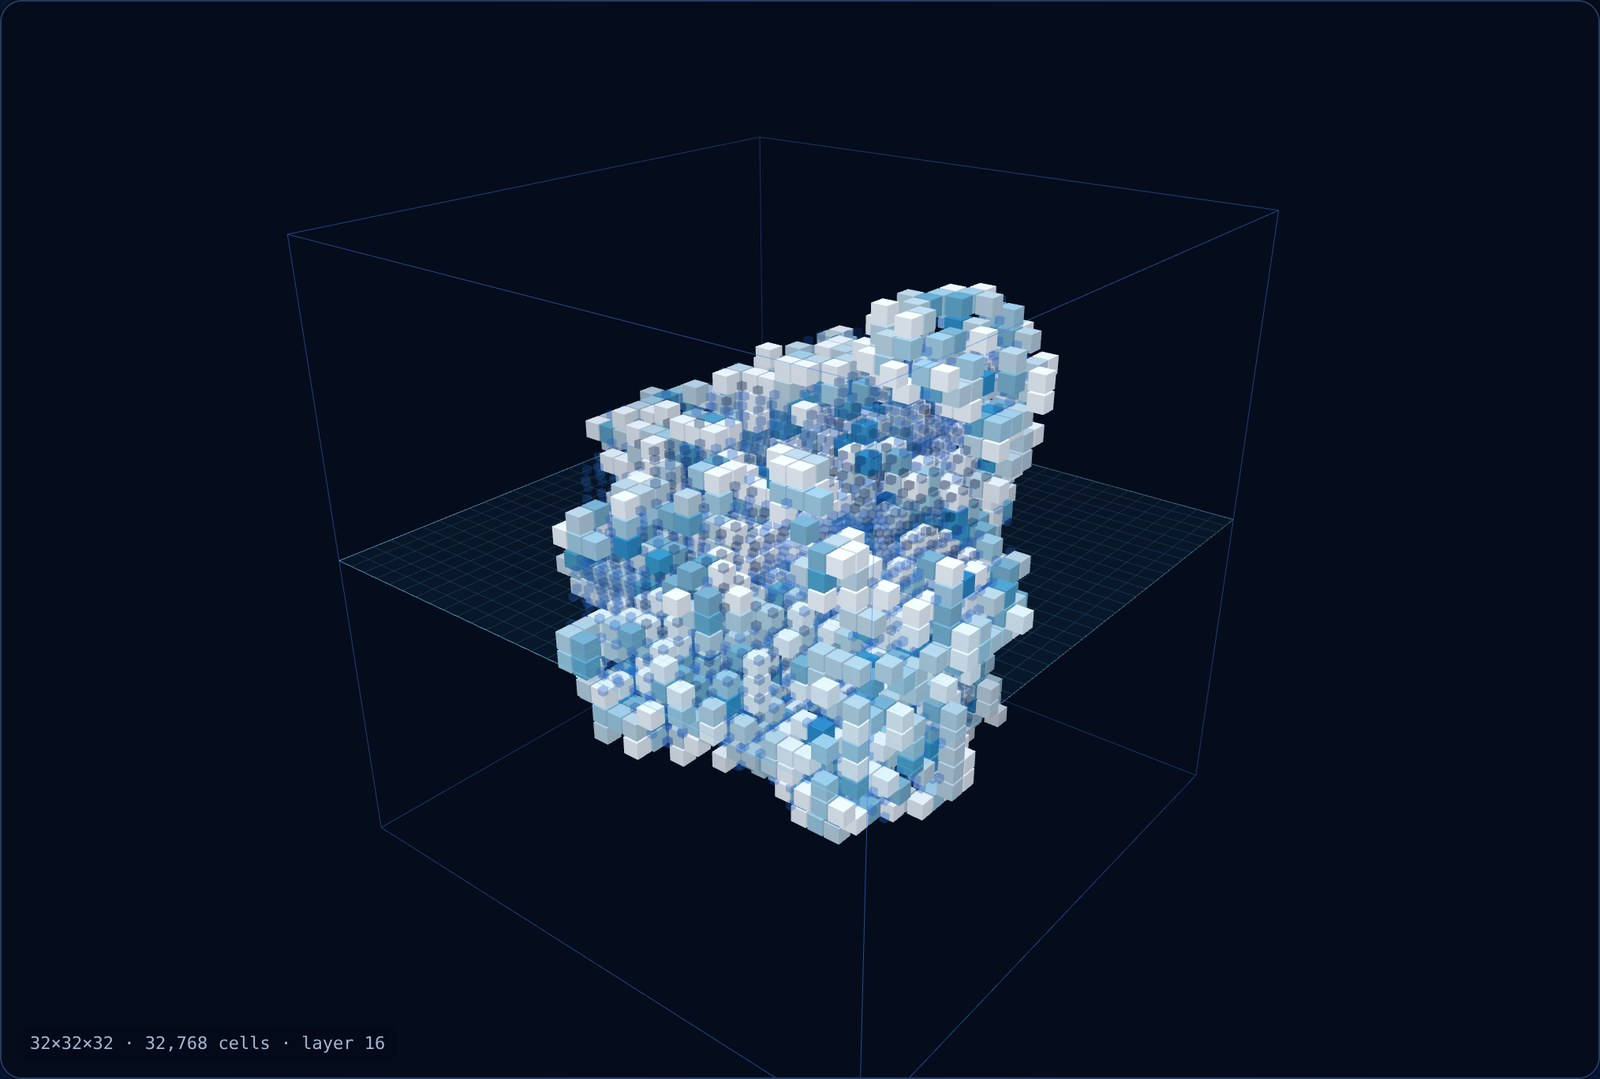
\includegraphics[width=\linewidth]{site_3d_amoeba.jpg}\caption{\rl{B6/S5678}: an ``amoeba'' growing from a small seed.}\end{subfigure}\hfill
  \begin{subfigure}[t]{0.49\linewidth}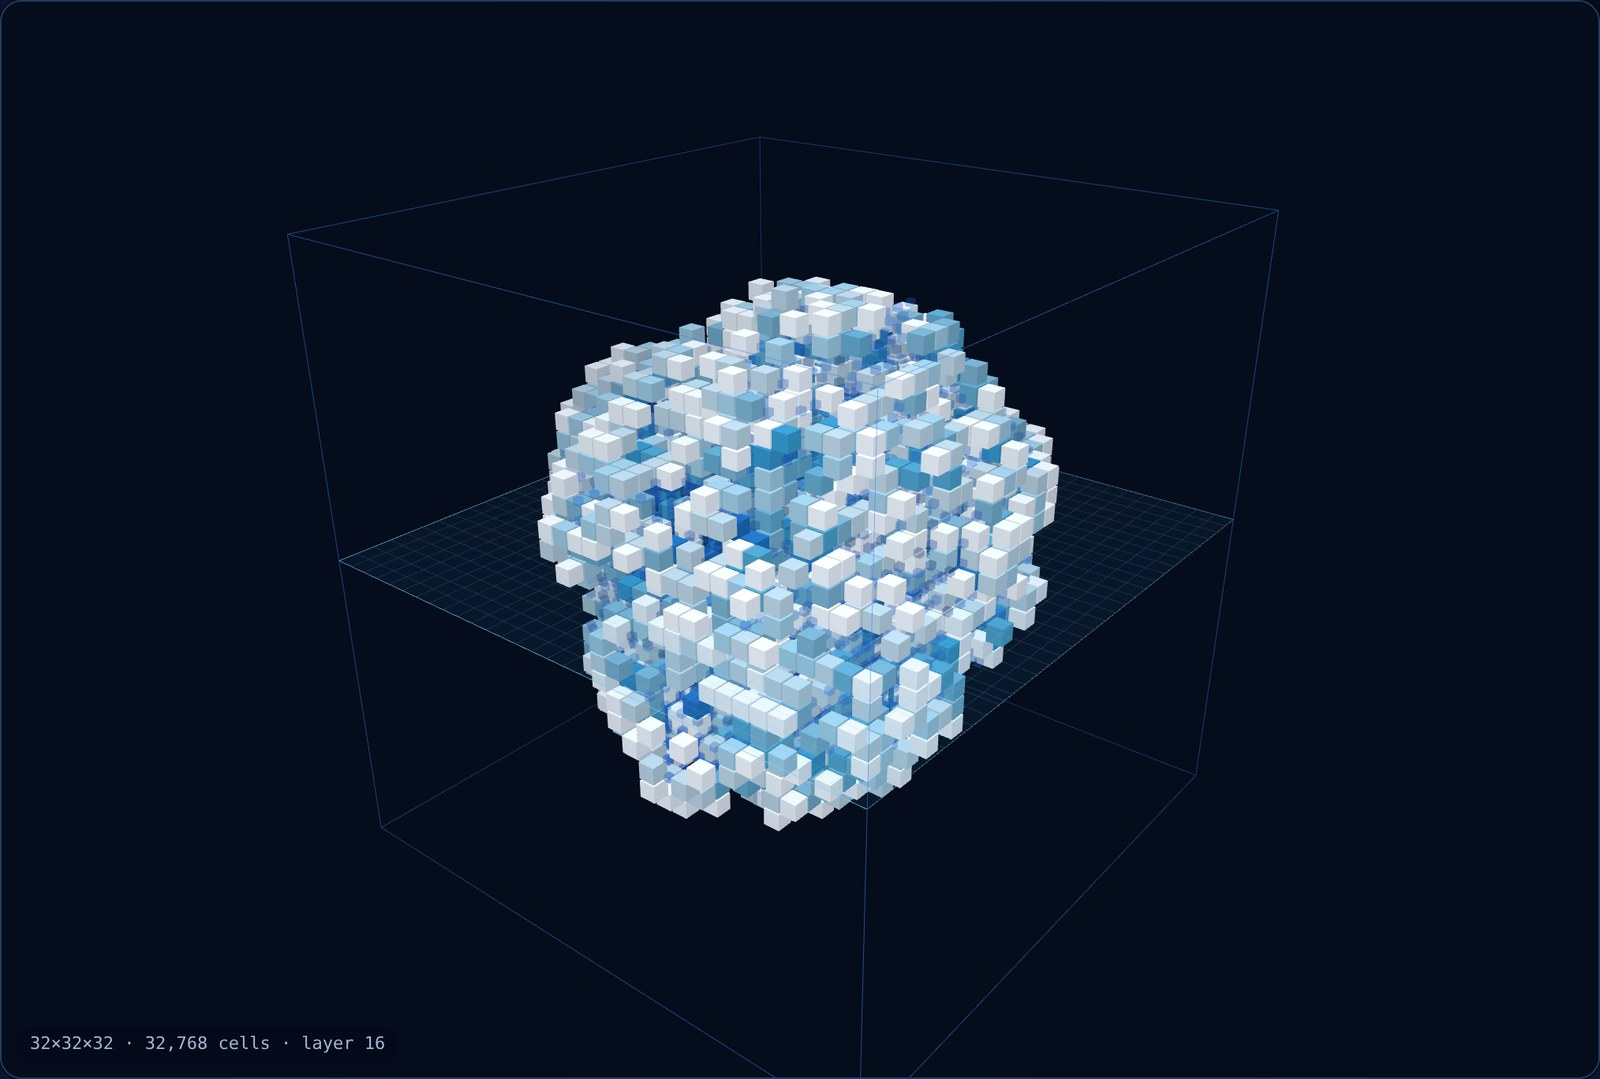
\includegraphics[width=\linewidth]{site_3d_crystal.jpg}\caption{\rl{B6/S45678}: grows into a ball that freezes solid.}\end{subfigure}\\[4pt]
  \begin{subfigure}[t]{0.49\linewidth}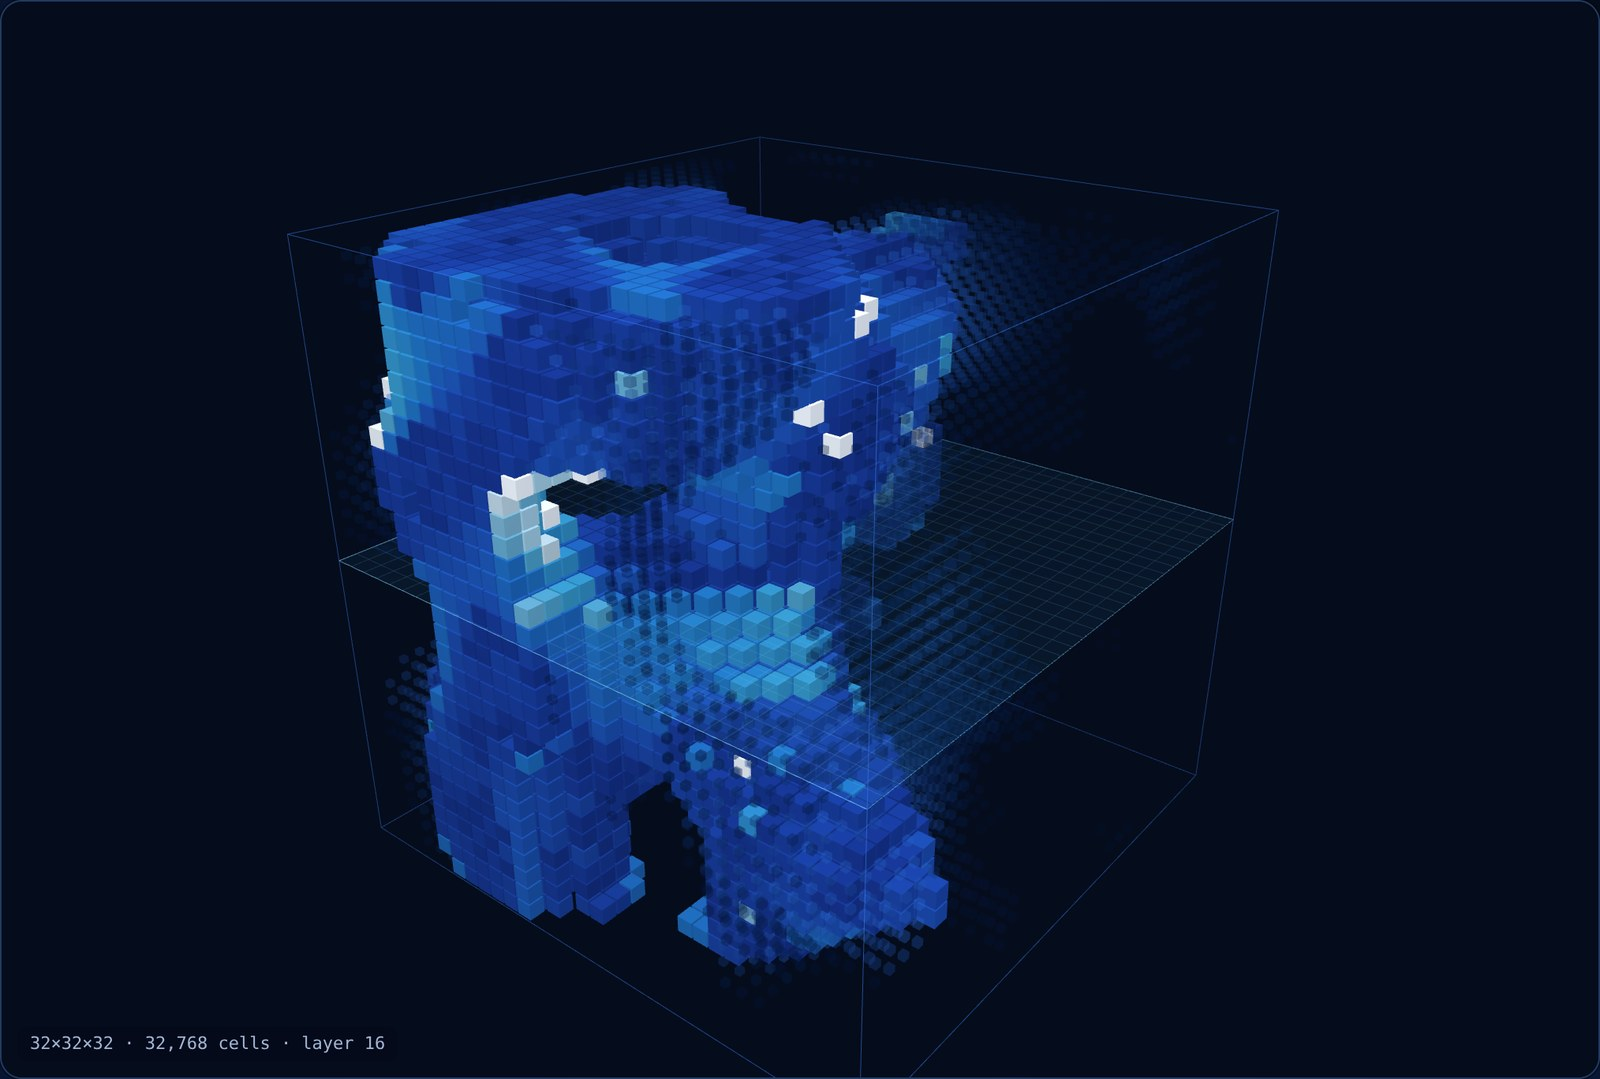
\includegraphics[width=\linewidth]{site_3d_clouds.jpg}\caption{``Clouds'' \rl{B13,14,17,18,19/S13--26}: a 50\% soup condenses into smooth, long-lived blobs (dark = old cells).}\end{subfigure}\hfill
  \begin{subfigure}[t]{0.49\linewidth}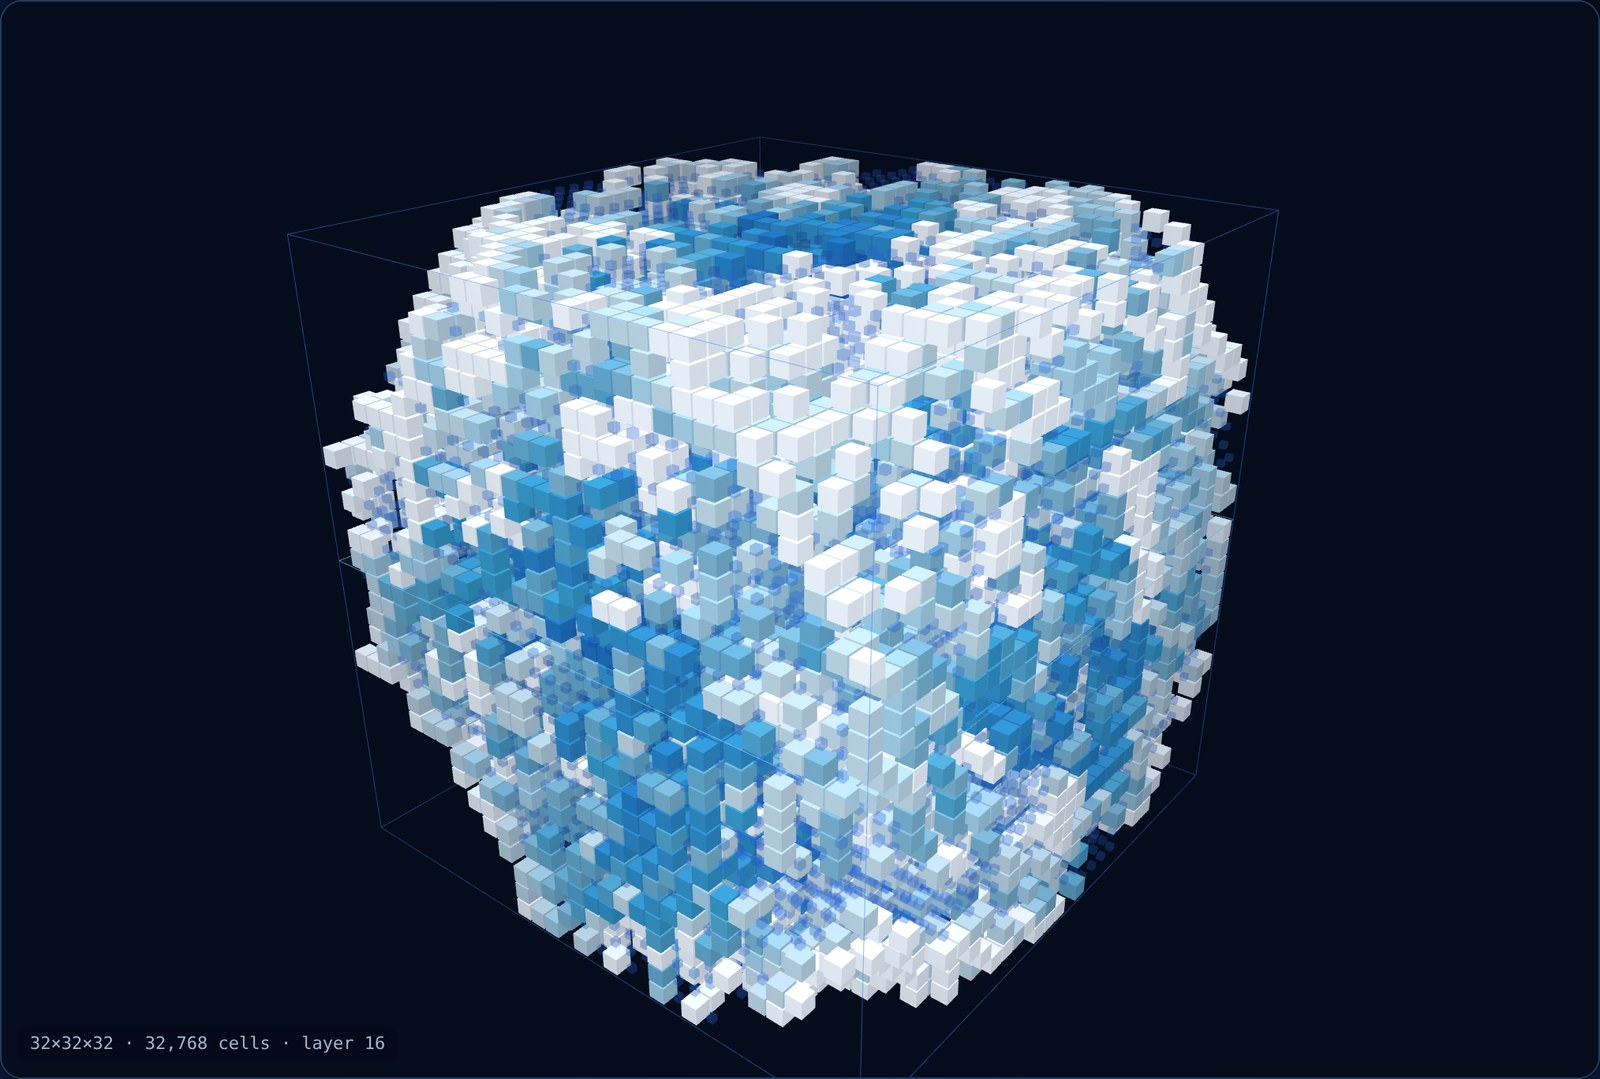
\includegraphics[width=\linewidth]{site_3d_coral.jpg}\caption{\rl{B567/S5--11}: coral-like growth that fills the grid.}\end{subfigure}
  \caption{3D rules on a $32^3$ torus, as shown on the website (white = newly born, dark blue = old).}
  \label{fig:3dsite}
\end{figure}

\subsection{How big can the 3D grid be?}

Figure~\ref{fig:timing} shows the time for one generation, measured natively on one core of a 2.1\,GHz Xeon.

\begin{itemize}
  \item \textbf{Compiler flags matter more than I expected.} With \texttt{-O3}, a 3D step costs about 22--24\,ns per cell, against 130--170\,ns with \texttt{-O2}: \textbf{5--7$\times$ faster}. The compiler unrolls the 27-iteration neighbour loop. The WebAssembly build (\texttt{-O3}) runs at about 29\,ns per cell in the browser engine, close to native.
  \item \textbf{Time is the limit, not memory.} The engine stores cells in \texttt{vector<bool>} (one bit each), so even $256^3$ (16.7 million cells) needs about 4\,MB for the two grids, plus 17\,MB for the byte copy made by \texttt{flatten()}. The \texttt{-O3} step times are $64^3$: 5.7\,ms; $128^3$: 51\,ms (about 20 generations per second); $256^3$: 0.39\,s.
  \item \textbf{In the browser, rendering is the limit.} The simulation could run $128^3$ at about 20 generations per second, but drawing up to two million cubes is too much for most GPUs. The website therefore stops at $64^3$, where both simulation and rendering keep up.
\end{itemize}

\yours{Run \texttt{./experiments/run timing} (compiled with \texttt{-O3}) on your own computer and replace these numbers, since the assignment asks about your machine. Also note the largest grid the website stays smooth on for you.}

\begin{figure}[!htbp]
  \centering
  \begin{minipage}[t]{0.49\linewidth}
    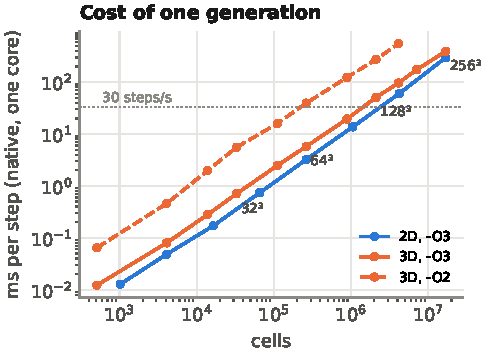
\includegraphics[width=\linewidth]{timing.pdf}
    \caption{Time per generation against grid size. Both axes are logarithmic.}
    \label{fig:timing}
  \end{minipage}\hfill
  \begin{minipage}[t]{0.49\linewidth}
    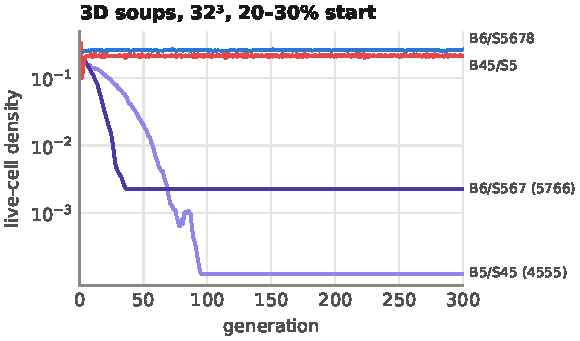
\includegraphics[width=\linewidth]{traces3d.pdf}
    \caption{3D soups on $32^3$ from a whole-grid random start ($d=0.2$ for B5/S45, B6/S567 and B45/S5; $0.3$ for B6/S5678). Log scale.}
    \label{fig:traces3d}
  \end{minipage}
\end{figure}

\subsection{Statistics of random 3D rules}

\paragraph{Uniform rules are all chaotic.} The 3D half of \texttt{main.cpp} continues the same random stream to draw 100 rules uniformly from all $2^{54}$. Each runs on $24^3$ for at most 200 generations from $d\in\{0.1,0.2,0.35\}$. \textbf{All 100 are chaotic}, with a median entropy of 0.97, and only 1 of 300 runs died out. The reason is the same as in 2D, but stronger. A rule avoids every birth count from 0 to 4 with probability $2^{-5}\approx3\%$. With 26 neighbours, a count of 4 or less is met by almost every dead cell in a 10--35\% soup, so almost every rule sets the whole grid boiling. In the sample, 94 of the 100 rules had a smallest birth count of 4 or less, and the other 6 had 5--8.

\paragraph{Sparser sampling.} To see the rest of 3D rule space, I sampled 100 rules where each count is included independently with probability $p=0.2$, and another 100 with $p=0.1$ (Figure~\ref{fig:3dcat}).

\begin{figure}[!htbp]
  \centering
  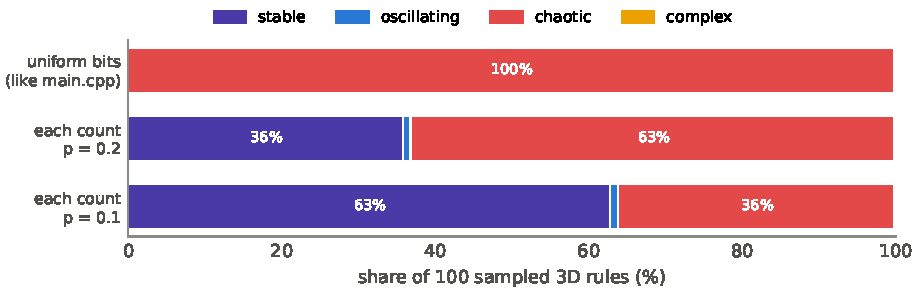
\includegraphics[width=\linewidth]{survey3d_categories.pdf}
  \caption{Categories of 100 random 3D rules ($24^3$, 200 generations) under three ways of sampling rules.}
  \label{fig:3dcat}
\end{figure}

\begin{center}\small
\begin{tabular}{@{}lccc@{}}
\toprule
Smallest birth count & uniform & $p=0.2$ & $p=0.1$ \\
\midrule
0 (B0)   & 47 chaotic & 20 chaotic, 1 oscillating & 7 chaotic \\
1--4     & 47 chaotic & 33 chaotic & 26 chaotic \\
5--8     & 6 chaotic  & 19 stable, 10 chaotic & 20 stable, 3 chaotic, 1 osc. \\
9 or more & --        & 17 stable & 39 stable \\
no birth & --         & -- & 4 stable \\
\bottomrule
\end{tabular}
\end{center}

\noindent The smallest birth count nearly decides the category on its own. \textbf{Every} rule with a birth count of 4 or less was chaotic (apart from one B0 strober), and \textbf{every} rule whose smallest birth count was 9 or more was stable, usually because it died out: 132 of the 300 $p=0.1$ runs ended with an empty grid. The interesting band is a smallest birth count of 5--8, where both outcomes happen. That is exactly where Carter Bays' 3D Life rules (\rl{B5/S45}, \rl{B6/S567}) sit. The classifier found \textbf{no} complex 3D rule in any of the three samples.

\paragraph{Comparing with 2D.}
\begin{itemize}
  \item \textbf{The critical birth count scales with the neighbourhood.} In 2D, rules become ``tame'' at birth count 3, which is $3/8=37.5\%$ of the neighbourhood. In 3D the band is 5--8, or 19--31\% of 26. In both cases a dead cell should need a fair fraction of its neighbours alive before it can be born.
  \item \textbf{Chaos is even more dominant in 3D} under uniform sampling (100\% against 76\%).
  \item \textbf{3D Life-like rules are fragile.} On the website and in Figure~\ref{fig:traces3d}, Bays' \rl{B5/S45} and \rl{B6/S567} usually collapse within about 100 generations, to a handful of small still lifes or to nothing. In a seed sweep, \rl{B5/S45} died completely in about half of the soups. Bays found gliders in these rules, but I never saw one arise from a random soup, whereas in Life gliders appear in almost every soup. The visually rich 3D rules (Figure~\ref{fig:3dsite}) are growth rules: amoebas, crystals, coral and clouds.
\end{itemize}

\yours{Add what you saw yourself in 3D: e.g.\ try building one of Bays' gliders in the 3D editor, or describe how the growth rules look while they run.}

%=====================================================================
\section{How I used AI}
%=====================================================================

\yours{Describe how you used AI when writing the C++ engine and classifier (\texttt{engine/}, \texttt{analysis/}): what you asked for, what you wrote or changed yourself, and how you checked it.}

\noindent The website and the analysis in this report were done with \textbf{Claude Code} (Anthropic's coding agent), working from my C++ engine and classifier and from the assignment text:
\begin{itemize}
  \item \textbf{Website.} It wrote the Emscripten bindings (\texttt{wasm/bindings.cpp}), including the \texttt{SeededGame} wrapper that lets the survey run in parallel while matching the CLI, and all of \texttt{web/}: the canvas viewer, the rule editor, the three.js 3D editor with ray-march picking, and the survey with its web workers and charts. It also wrote the GitHub Pages workflow. My instructions were the design brief: a blue colour scheme with recently changed cells in white, clickable rule editing, a 3D mode with a real 3D editor, and a survey section that feeds the viewer. I also told it not to modify my C++.
  \item \textbf{Checking.} Before building the interface, it compiled my engine natively and to WebAssembly and confirmed that both give identical survey results (same rules, labels and entropies as \texttt{main.cpp}). It tested the site in a headless browser, including drawing, 3D clicks, survey runs and replay, and phone-width layout.
  \item \textbf{Experiments and report.} It wrote \texttt{experiments/experiments.cpp}, which uses the engine and \texttt{Analysis} unchanged, and \texttt{experiments/figures.py}, ran them, and drafted this report. Along the way it verified several claims instead of assuming them: the replicator formula (25/25 checkpoints), the B0 strobe equivalence (4000/4000 generations), that Life's glider also works in HighLife, and that the 3D presets on the website survive across seeds (two didn't, and were fixed).
  \item \textbf{Things it caught.} \texttt{main.cpp} referenced a \texttt{TrialResult::activeEntropy} field that doesn't exist in \texttt{analysis.hpp}. A first version of the object census counted each half of a split toad as an unknown object. And the \texttt{-O2} vs.\ \texttt{-O3} gap in the timing.
\end{itemize}

%=====================================================================
\section{Limitations}
%=====================================================================

\begin{itemize}
  \item \textbf{Finite torus.} Gliders can't escape, so soups on a torus settle differently from soups on an infinite plane. The ash statistics are for $128\times128$.
  \item \textbf{Finite time.} Labels depend on \texttt{maxGen}. \rl{B45678/S12358} is complex at 500 generations and oscillating by about 900. Four Life soups were still active at 6000.
  \item \textbf{The entropy threshold (0.35) was chosen by hand} for 2D and reused unchanged for 3D. No 3D rule was labelled complex, which may say as much about the measure as about 3D rules.
  \item \textbf{Strobing B0 rules} fool the entropy measure (Section~\ref{sec:strobe}), and whole-grid hashing can't see a glider travelling through otherwise still debris.
  \item \textbf{Three runs per rule} isn't much: 6\% of 2D rules got different labels from different densities.
  \item \textbf{Sample sizes}: 100 rules per 3D sampling scheme, and one grid size ($24^3$) for the 3D survey.
  \item \textbf{Performance}: the engine counts neighbours cell by cell with modulo wrap-around. Bit-parallel or GPU methods would allow much larger grids, and the browser view is capped at $64^3$ by rendering.
\end{itemize}

%=====================================================================
\section{Thoughts}
%=====================================================================

\yours{Your own reflections: what excited you, what surprised you, and what you'd like to learn more about. Some threads from this project you could pick up: the replicator following the Sierpinski triangle (a 2D rule reproducing a 1D rule); how rare ``complex'' is and how hard it is to measure; the smallest birth count working as a phase boundary in both 2D and 3D; and the link to the Emergent Garden video's question of what makes a system life-like (reproduction, as in the replicator; variation and selection, which these deterministic rules don't have).}

\clearpage
\appendix
%=====================================================================
\section{All 100 sampled 2D rules}\label{app:table}
%=====================================================================

Seed 2026, $64\times64$, 500 generations. The same list as \texttt{main.cpp} and the website survey produce. Each run cell is the run's label (S = stable, O = oscillating, X = chaotic, C = complex) followed by either the period and generation of the first repeat ($p$\,period\,@\,generation) or the mean entropy ($H$). $^\dagger$ marks runs that died out.

{\small
\begin{longtable}{@{}rllccc@{}}
\toprule
\# & Rule & Label & $d=0.20$ & $d=0.35$ & $d=0.50$ \\
\midrule
\endhead
1 & \texttt{B02358/S34578} & chaotic & X H0.93 & X H0.93 & X H0.93 \\
2 & \texttt{B3/S12567} & chaotic & X H0.72 & X H0.54 & X H0.76 \\
3 & \texttt{B0467/S02468} & chaotic & X H0.85 & X H0.85 & X H0.84 \\
4 & \texttt{B13567/S156} & chaotic & X H0.96 & X H0.96 & X H0.96 \\
5 & \texttt{B146/S01256} & chaotic & X H0.95 & X H0.95 & X H0.95 \\
6 & \texttt{B03468/S12346} & chaotic & X H0.93 & X H0.93 & X H0.93 \\
7 & \texttt{B2347/S057} & chaotic & X H0.96 & X H0.96 & X H0.96 \\
8 & \texttt{B02345/S356} & chaotic & X H0.93 & X H0.93 & X H0.93 \\
9 & \texttt{B4568/S147} & stable & S p1@7 & S p1@13 & O p2@18 \\
10 & \texttt{B24678/S27} & chaotic & X H0.92 & X H0.93 & X H0.92 \\
11 & \texttt{B034/S1457} & chaotic & X H0.97 & X H0.97 & X H0.97 \\
12 & \texttt{B0467/S2347} & chaotic & X H0.95 & X H0.96 & X H0.96 \\
13 & \texttt{B0123458/S023467} & chaotic & X H0.86 & X H0.86 & X H0.86 \\
14 & \texttt{B01347/S14567} & oscillating & O p60@107 & O p4@62 & O p6@42 \\
15 & \texttt{B235/S0123456} & oscillating & O p2@14 & O p2@15 & O p6@20 \\
16 & \texttt{B04567/S2568} & chaotic & X H0.88 & X H0.88 & X H0.88 \\
17 & \texttt{B013457/S037} & chaotic & X H0.96 & X H0.96 & X H0.96 \\
18 & \texttt{B1256/S35678} & stable & S p1@18 & S p1@16 & S p1@17 \\
19 & \texttt{B013468/S036} & chaotic & X H0.97 & X H0.97 & X H0.97 \\
20 & \texttt{B23678/S078} & chaotic & X H0.90 & X H0.90 & X H0.90 \\
21 & \texttt{B017/S4678} & chaotic & X H0.87 & X H0.87 & X H0.87 \\
22 & \texttt{B2367/S012345} & chaotic & X H0.92 & X H0.92 & X H0.92 \\
23 & \texttt{B01234568/S12367} & chaotic & X H0.90 & X H0.90 & X H0.90 \\
24 & \texttt{B03467/S124568} & chaotic & X H0.82 & X H0.82 & X H0.82 \\
25 & \texttt{B02345/S1468} & chaotic & X H0.94 & X H0.94 & X H0.94 \\
26 & \texttt{B234/S04} & chaotic & X H0.94 & X H0.94 & X H0.94 \\
27 & \texttt{B1345/S012368} & chaotic & X H0.94 & X H0.94 & X H0.94 \\
28 & \texttt{B04578/S0368} & chaotic & X H0.83 & X H0.84 & X H0.84 \\
29 & \texttt{B4578/S0234678} & oscillating & X H0.52 & O p2@52 & O p2@28 \\
30 & \texttt{B0123458/S48} & chaotic & X H0.85 & X H0.85 & X H0.85 \\
31 & \texttt{B01378/S024568} & chaotic & X H0.96 & X H0.96 & X H0.96 \\
32 & \texttt{B01237/S1238} & chaotic & X H0.88 & X H0.87 & X H0.88 \\
33 & \texttt{B348/S03458} & chaotic & X H0.96 & X H0.96 & X H0.96 \\
34 & \texttt{B12378/S356} & chaotic & X H0.96 & X H0.96 & X H0.96 \\
35 & \texttt{B12467/S0235678} & stable & S p1@11 & S p1@10 & S p1@10 \\
36 & \texttt{B014578/S012457} & chaotic & X H0.92 & X H0.92 & X H0.92 \\
37 & \texttt{B02678/S246} & chaotic & X H0.92 & X H0.92 & X H0.92 \\
38 & \texttt{B056/S67} & chaotic & X H0.74 & X H0.74 & X H0.74 \\
39 & \texttt{B0457/S023578} & chaotic & X H0.95 & X H0.95 & X H0.95 \\
40 & \texttt{B1568/S01246} & chaotic & X H0.87 & X H0.88 & X H0.86 \\
41 & \texttt{B0178/S0348} & chaotic & X H0.94 & X H0.94 & X H0.94 \\
42 & \texttt{B023468/S014678} & oscillating & O p2@93 & O p2@119 & S p1@132 \\
43 & \texttt{B02567/S012367} & chaotic & X H0.97 & X H0.97 & X H0.97 \\
44 & \texttt{B024567/S178} & oscillating & O p2@64 & O p2@50 & O p2@57 \\
45 & \texttt{B01458/S1568} & chaotic & X H0.93 & X H0.93 & X H0.93 \\
46 & \texttt{B04568/S58} & chaotic & X H0.78 & X H0.78 & X H0.78 \\
47 & \texttt{B0134678/S0127} & chaotic & X H0.95 & X H0.95 & X H0.95 \\
48 & \texttt{B678/S124567} & stable & S p1@6 & S p1@13 & O p2@28 \\
49 & \texttt{B23578/S013456} & chaotic & X H0.86 & X H0.86 & X H0.86 \\
50 & \texttt{B026/S023} & chaotic & X H0.92 & X H0.92 & X H0.92 \\
51 & \texttt{B123467/S013678} & oscillating & O p12@181 & O p6@191 & O p4@230 \\
52 & \texttt{B0123457/S012468} & chaotic & X H0.91 & X H0.91 & X H0.91 \\
53 & \texttt{B24567/S0124678} & stable & S p1@19 & O p4@19 & S p1@16 \\
54 & \texttt{B01257/S23478} & chaotic & X H0.97 & X H0.97 & X H0.97 \\
55 & \texttt{B012467/S047} & chaotic & X H0.96 & X H0.96 & X H0.96 \\
56 & \texttt{B0457/S345} & chaotic & X H0.94 & X H0.94 & X H0.94 \\
57 & \texttt{B0234/S024567} & oscillating & O p12@23 & O p12@32 & O p6@24 \\
58 & \texttt{B03467/S2568} & chaotic & X H0.95 & X H0.95 & X H0.95 \\
59 & \texttt{B014567/S012345} & chaotic & X H0.89 & X H0.88 & X H0.88 \\
60 & \texttt{B1248/S0568} & chaotic & X H0.94 & X H0.94 & X H0.94 \\
61 & \texttt{B1246/S237} & chaotic & X H0.94 & X H0.94 & X H0.94 \\
62 & \texttt{B0345/S167} & chaotic & X H0.96 & X H0.96 & X H0.96 \\
63 & \texttt{B0678/S17} & oscillating & O p120@303 & O p120@416 & X H0.79 \\
64 & \texttt{B0123567/S0123567} & chaotic & X H0.75 & X H0.75 & X H0.75 \\
65 & \texttt{B012378/S013} & oscillating & O p2@8$^\dagger$ & O p2@24 & O p2@43 \\
66 & \texttt{B3456/S01345678} & stable & S p1@10 & S p1@6 & S p1@4 \\
67 & \texttt{B1678/S012345} & oscillating & O p4@24 & O p4@19 & O p4@16 \\
68 & \texttt{B256/S168} & chaotic & X H0.85 & X H0.85 & X H0.85 \\
69 & \texttt{B023467/S12347} & chaotic & X H0.90 & X H0.90 & X H0.90 \\
70 & \texttt{B012468/S013478} & chaotic & X H0.96 & X H0.96 & X H0.96 \\
71 & \texttt{B02345/S23457} & chaotic & X H0.83 & X H0.84 & X H0.83 \\
72 & \texttt{B123467/S135} & chaotic & X H0.92 & X H0.92 & X H0.92 \\
73 & \texttt{B037/S2458} & chaotic & X H0.95 & X H0.95 & X H0.95 \\
74 & \texttt{B027/S01268} & chaotic & X H0.87 & X H0.87 & X H0.87 \\
75 & \texttt{B01578/S0145} & chaotic & X H0.90 & X H0.90 & X H0.90 \\
76 & \texttt{B1368/S246} & chaotic & X H0.96 & X H0.96 & X H0.96 \\
77 & \texttt{B067/S0178} & oscillating & O p6@16 & O p6@22 & O p6@23 \\
78 & \texttt{B15678/S1268} & chaotic & X H0.88 & X H0.89 & X H0.89 \\
79 & \texttt{B012467/S23567} & chaotic & X H0.81 & X H0.80 & X H0.80 \\
80 & \texttt{B1678/S0137} & oscillating & O p12@442 & O p72@358 & X H0.86 \\
81 & \texttt{B034567/S125678} & stable & S p1@10 & S p1@8 & S p1@8 \\
82 & \texttt{B02567/S013568} & chaotic & X H0.91 & X H0.91 & X H0.91 \\
83 & \texttt{B1247/S03456} & chaotic & X H0.91 & X H0.91 & X H0.91 \\
84 & \texttt{B3468/S1467} & chaotic & X H0.97 & X H0.96 & X H0.97 \\
85 & \texttt{B13478/S0347} & chaotic & X H0.96 & X H0.96 & X H0.96 \\
86 & \texttt{B457/S06} & stable & S p1@4 & S p1@7 & S p1@8 \\
87 & \texttt{B3578/S0234678} & oscillating & O p2@52 & O p4@47 & O p2@44 \\
88 & \texttt{B0123458/S13456} & oscillating & O p2@17 & O p2@17 & O p2@33 \\
89 & \texttt{B015/S02367} & chaotic & X H0.92 & X H0.92 & X H0.92 \\
90 & \texttt{B4/S1234678} & oscillating & X H0.97 & O p30@187 & O p36@218 \\
91 & \texttt{B13567/S04678} & oscillating & O p4@38 & O p4@40 & O p4@38 \\
92 & \texttt{B135/S012357} & chaotic & X H0.96 & X H0.96 & X H0.96 \\
93 & \texttt{B078/S0278} & oscillating & O p6@26 & O p6@21 & O p6@29 \\
94 & \texttt{B012367/S35} & complex & O p2@272 & C H0.13 & C H0.22 \\
95 & \texttt{B012458/S34568} & oscillating & O p6@86 & O p24@133 & O p60@174 \\
96 & \texttt{B45/S148} & stable & S p1@9 & S p1@10 & S p1@11 \\
97 & \texttt{B012367/S04678} & oscillating & O p16@80 & O p16@346 & O p16@326 \\
98 & \texttt{B045678/S02456} & chaotic & X H0.88 & X H0.88 & X H0.88 \\
99 & \texttt{B013/S02456} & chaotic & X H0.96 & X H0.96 & X H0.97 \\
100 & \texttt{B1235678/S2467} & chaotic & X H0.84 & X H0.84 & X H0.84 \\
\bottomrule
\end{longtable}
}


\end{document}
